\documentclass[a4aper,12pt]{report}
\usepackage[margin=1in]{geometry}
%For Drawing 
%tikzpicture
\usepackage{tikz}
\usepackage{scalerel}
\usepackage{pict2e}
\usepackage{tkz-euclide}
\usetikzlibrary{calc}
\usetikzlibrary{patterns,arrows.meta}
\usetikzlibrary{shadows}
\usetikzlibrary{external}
\usetikzlibrary{intersections}
\usetikzlibrary{shapes.geometric, arrows}
\usepackage[american,RPvoltages]{circuitikz}
\ctikzset{
    resistors/scale=0.6    
}
%Hyperlinking Texts and Others
\usepackage{hyperref}
\hypersetup{
    colorlinks = true,
    linkcolor=black,
    urlcolor=black,
    pdftitle = {MAT-2101: Ordinary and Partial Differential
Equations}
}
%Header and Footer
\usepackage{fancyhdr}
\pagestyle{fancy}
\lhead{MAT-2101: Ordinary and Partial Differential
Equations}
\rhead{Note by \href{https://www.facebook.com/nosrat.jahan.romy}{Romy} \& \href{https://www.facebook.com/mdgalibashrafbd}{Galib}}


\usepackage{fancyvrb}
\usepackage{lipsum}
\usepackage{array}
%For creating boxes and others fancy
\usepackage[most,many]{tcolorbox}
\tcbuselibrary{xparse}
\tcbuselibrary{listings, breakable}
% Define custom tcolorbox style for question and solution

\newtcolorbox{hw}[1][]{
  title=\textbf{H.W: }~#1,
  coltitle=white,
  colback=blue!5,
  colframe=blue!60!black,
  colbacktitle=blue!30!black,
  breakable,
  enhanced,
  boxrule=1pt,
  arc=4pt, % custom curvature for difference
  top=6pt,
  bottom=6pt,
  left=8pt,
  right=8pt,
  before upper={\stepcounter{examplebox}}
}
%pgfplots
\usepackage{pgfplots}
\pgfplotsset{compat=newest}
\usepgfplotslibrary{statistics}
\usepgfplotslibrary{fillbetween}

%To add color in texts
\usepackage{xcolor}

%For using correct symbols and others by default
\usepackage{amsmath, amssymb, amsfonts}

%For Styling Chapters title
%Options: Sonny, Lenny, Glenn, Conny, Rejne, Bjarne, Bjornstrup
\usepackage[Conny]{fncychap}

\usepackage{enumitem}

\usepackage{array,tabularx}
\usepackage{colortbl}
\usepackage{changepage}
\renewcommand{\arraystretch}{1.5}
\usepackage{graphicx}
\usepackage{wrapfig}
\begin{document}
\pgfplotsset{
    standard/.style={
    axis line style = thick,
    trig format=rad,
    enlargelimits,
    axis x line=middle,
    axis y line=middle,
    enlarge x limits=0.15,
    enlarge y limits=0.15,
    every axis x label/.style={at={(current axis.right of origin)},anchor=north west},
    every axis y label/.style={at={(current axis.above origin)},anchor=south east}
    }
}
    \begin{center}
        \begin{LARGE}
            \textbf{\noindent Department of Electrical and Electronics Engineering} \\
             \textbf{University of Dhaka} \\
        \end{LARGE}
        \begin{Large}
        Batch - 103, EEE-58 \\
        \end{Large}
        \vspace{1.5cm}
        \begin{Large}
            $2^{nd}$ Year $1^{st}$ Semester \\ 
        \end{Large}
        \vspace{1.5cm}
        
\includegraphics[scale=0.5]{logo.du.png} \\
        \vspace{0.5cm}
    \end{center}
    \begin{Large}
         \noindent\textbf{Course: MAT-2101} \\ 
        \textbf{Title: Ordinary and Partial Differential
Equations}\\
        Class Teacher: Md. Motaleb Hossen\\
    \end{Large}
    \vspace{0.5cm}
    \begin{center}
        {\Large\textbf{ Note by}} \\
        \begin{minipage}{0.3\linewidth}
            \begin{flushright}
                {\large
                Nosrat Jahan Romy \\
        Session: 2023-2024 \\ 
        Class Roll: RH-041}
            \end{flushright}
        \end{minipage}
        \begin{minipage}{0.05\linewidth}
            \begin{center}
                \rule{1pt}{2.2cm}
            \end{center}
            
        \end{minipage}
        \begin{minipage}{0.3\linewidth}
            {\large Md. Galib Ashraf \\
        Session: 2023-2024 \\ 
        Class Roll: SH-042}
        \end{minipage}
    \begin{Large}
         
        
    \end{Large}    
    \end{center}
    \thispagestyle{empty}
    \newpage 
    \chapter*{Syllabus}
    \vspace*{-2.7cm}
    \textbf{Ordinary Differential Equations (ODEs)} \\ [5pt] 
    \textbf{First-order ODE: }General Form of Solution, First-degree First-order Equations, Separable-variable Equations, Exact Equations, Inexact Equations, Integrating Factors, Linear Equations, Homogeneous Equations, Isobaric Equations, Bernoulli’s Equation, Existence and Uniqueness of Solutions for Initial Value Problems, Higher-Degree First-Order Equations, Clairaut’s Equation. \\ [5pt]
    \textbf{Second-Order ODEs: }Homogeneous Linear ODEs of Second Order, Homogeneous Linear ODEs with Constant Coefficient, Euler–Cauchy Equations, Existence and Uniqueness of Solutions, Wronskian, Nonhomogeneous ODEs, Method of Undetermined Coefficients, Solution by Variation of Parameters. \\ [5pt]
    \textbf{Series Solutions of ODEs: }Power Series Method, Legendre’s Equation and Legendre Polynomials, Bessel’s Equation and Bessel Functions, Laguerre Differential Equation and Laguerre Polynomials, Airy Differential Equation, Hermite Differential Equation and Hermite Differential Polynomials. \\ [8pt]\textbf{Partial Differential Equations (PDEs)} \\ [5pt] 
    \textbf{Important Partial Differential Equations: }The Wave Equation, The Diffusion Equation, Laplace Equation, Poisson’s Equations, Schrodinger’s Equation. \\ [5pt]
    \textbf{Solving PDEs: }General and Particular Solutions, Separation of Variables, Superposition of Separated Solutions, Separation of Variables in Polar Coordinates, Laplace Equation in Polar Coordinates, Spherical Harmonics, Helmholtz’s Equation, Integral Transform Methods, Inhomogeneous PDE Problems with Green’s Functions Approach.
\newpage
\chapter*{Reference Books}
\vspace*{-2.7cm}
\thispagestyle{empty}
\begin{enumerate}
    \item Mathematical Methods for Physics and Engineering, $3^{rd}$ Edition, K. F. Riley, M. P. Hobson, and S. J. Bence, Cambridge University Press.
    \item Advanced Engineering Mathematics, $10^{th}$ Edition, Erwin Kreyszigm Herbert Kreyszig and Edward J. Norminton, John-Wiley and Sons.
    \item Mathematical Method for Physicist, $6^{th}$ Edition, George B. Arfken and Hans J. Weber, Elsevier Academic Press.
    \item Schaum's Outline of Advanced Mathematics for Engineers and Scientists, $1^{st}$ Edition, Murray R. Spiegel, McGraw Hill.
    \item Schaum's Outline of Differential Equations, $4^{th}$ Edition, Richard Bronson and Gabriel Costa, McGraw Hill.
    \item Schaum's Outline of Partial Differential Equations, $3^{rd}$ Edition, Paul Du Chateau and D. W. Zachmann, McGraw Hill.
\end{enumerate}
\tableofcontents 
\thispagestyle{empty}
\newpage
\setcounter{page}{1}
\chapter{Differential Equations}
\vspace*{-30pt}
\textbf{Differential Equation: }An equation involving derivative or differentials of one or more dependent variables with respect to one or more independent variable, is called a differential equation. Example: 
\begin{align*}
    \dfrac{dy}{dx} + y = 0\qquad\qquad & y = f(x) \\ 
    \dfrac{d^2y}{dx^2}+\dfrac{dy}{dx}+6y=0 \qquad\qquad& [\text{dependent}\rightarrow 1(y),\text{independent} \rightarrow 1(x) ] \\ 
    \dfrac{du}{dx} +\dfrac{dv}{dy} = 0 \qquad\qquad & [\text{dependent} \rightarrow 2(u,v), \text{independent} \rightarrow 2(x,y)]
\end{align*}
\textbf{Ordinary Differential Equation: } A differential equation involving ordinary derivatives one or more dependent variables with respect to a single independent variable is called Ordinary Differential Equation (ODE). Example: \\ 
   \begin{adjustwidth}{2cm}{5pt}
        $\bullet\,\,\dfrac{d^2y}{dx^2} + \dfrac{dy}{dx} + y = 0$ \\ [5pt]
        $\bullet\,\,\dfrac{dy}{dx}+\dfrac{dz}{dx} = 0$ \\ [5pt]
        $\bullet\,\,\dfrac{dy}{dx} = x+\sin x \Rightarrow dy = (x+\sin x)dx$
    \end{adjustwidth}
    \vspace*{10pt}
    \textbf{Partial Differential Equation: } A differential equation involving partial derivatives of one or more dependent variables with respect to more than one independent variable is called Partial Differential Equation (PDE). Example:
    \vspace*{5pt}  
    \begin{adjustwidth}{2cm}{5pt}
        $\bullet \, \, \dfrac{d^2u}{dx^2} + \dfrac{d^2u}{dy^2}= 0$ \\ [5pt]
        $\bullet \,\,\dfrac{du}{dx}=-\dfrac{dv}{dy}$ 
    \end{adjustwidth}
    \vspace*{10pt}
    \textbf{Order of Differential Equation: }The order of a differential equation is the highest ordered derivate involved in the differential equation is called the order of this differential equation. Example: 
    \begin{align*}
        \dfrac{d^2y}{dx^2}+ \left(\dfrac{dy}{dx}\right)^2 = 0 \qquad &\longrightarrow \qquad \text{order} = 2 \\ 
        \dfrac{dy}{dx}+y = 0\qquad &\longrightarrow \qquad \text{order} = 1
    \end{align*}
    \vspace*{10pt}
    \textbf{Degree of Differential Equation: } The degree of a differential equation is the degree of the highest derivatives which occurs in its. Example: 
    \begin{align*}
        \left(\dfrac{d^2y}{dx^2}\right)^1+\left(\dfrac{dy}{dx}\right)^3=0 \qquad &\longrightarrow \quad \text{Degree = }(1) \\ 
        \left(\dfrac{d^3y}{dx^3}\right)^3+\left(\dfrac{dy}{dx}\right)^4=0 \qquad &\longrightarrow \quad \text{Degree = }(3) \\ 
    \end{align*}
    \textbf{Linear Differential Equation: } A differential equation is called linear if \begin{enumerate}
        \item Every dependent variables and every derivatives involved occur in the $1^{st}$ degree only. 
        \item No product of dependent variables and\textbackslash or derivatives 
    \end{enumerate}
    A differential equation which doesn't follow the following rules is a non-linear equation.
    Example: 
    \begin{equation*}
   \text{Liner Differential Equation} \longrightarrow \left\{
   \begin{array}{c}
     \dfrac{d^2y}{dx^2}+5\dfrac{dy}{dx}+6y=0 \\ [10pt] 
     \dfrac{d^4y}{dx^4}+x\dfrac{dy}{dx}+6x^2=0 
   \end{array}
   \right.
\end{equation*}
\begin{equation*}
   \text{Non-Liner Differential Equation} \longrightarrow \left\{
   \begin{array}{c}
     \dfrac{d^2y}{dx^2}+5\dfrac{dy}{dx}+y^2=0 \\ [10pt] 
     \dfrac{d^2y}{dx^2}+y\dfrac{dy}{dx}+e^x=0 
   \end{array}
   \right.
\end{equation*}
\textbf{\large Solution of Differential Equation: }\\ [7pt]
If $y=f(x)$ satisfy the equation of $\dfrac{dy}{dx}$ then $y$ is the solution of $\dfrac{dy}{dx}$. Example: 
\begin{align*}
    & \dfrac{dy}{dx}\,\, =\,\, x \\
    \Rightarrow  \,\,& dy\,\, =\,\, xdx \\
    \Rightarrow\,\, & \int dy\,\, = \,\,\int xdx \\ 
    \Rightarrow\,\,  & y \,\,= \,\,\dfrac{x^2}{2}+c \qquad (\text{Ans})
\end{align*}
$\bullet\,\,$ Consider the $n^{th}$ order differential equation in one dependent variable
$$F(x,y,y',y'',.....,y^n) = 0$$
$$a_0\dfrac{d^ny}{dx^n}+a_1\dfrac{d^{n-1}y}{dx^{n-1}}+a_2\dfrac{d^{n-2}y}{dx^{n-2}}+\cdots \cdots +a_n\dfrac{dy}{dx}+y+x= 0$$
Where, $F$ is a real valued function of n+2 variables $x,y,y',y'',\cdots,y^n$ and where $y^n=\dfrac{d^ny}{dx^n}$ \\ [5pt]
Any relation between dependent and independent variables which when substituted in the differential equation reduces it to an identity  is called a solution of differential equation. \\ [3pt]
For example: if $\dfrac{dy}{dx} = x$, then the solution of this differential equation is $y=\dfrac{x^2}{2}+c$ which is the relation between the dependent variable $y$ and independent variable $x$. 
\begin{flushright}
    {\small \textbf{End of Class 01 (12 Aug,2025)}}
\end{flushright}
\begin{equation}
    F(x,y,y',y'',.....,y^n) = 0
\end{equation}
Let $f$ be a real valued function defined for all $x$ ina a real interval $I$ and having $n$ derivatives for all $x\in I$, that are continuous on $I$. Then function $f$ is called an explicit solution of the equation (1.1) on $I$ if 
\begin{enumerate}
    \item $F(x,f,f',f'',.....,f^n)$ is defined for all $x\in F$
    \item $F(x,f,f',f'',.....,f^n) = 0$ for all $x\in I$
\end{enumerate}

That is the substitution of $f$ and its derivatives in equation (1.1) reduce (1.1) to an identity on $I$.
\begin{tcolorbox}[breakable, title=\textbf{Example 1.1: }]
     $$y=\sin x +c \,\,\, \text{is the solution of } \dfrac{d^2y}{dx^2}+\sin x=0$$.
     \vspace*{-5pt}
\end{tcolorbox}
\vspace*{5pt}
\noindent \textbf{Implicit Solution : } \\ [5pt]
A relation  $g(x,y)=0$ is called an implicit solution of (1.1) if this relation defines at least one real function $f$ of the variable $x$ on $I$ and that $f$ is an implicit  solution of (1.1) on the interval.
\begin{tcolorbox}[breakable,
    title={\textbf{Example 1.2: }The relation $x^2+y^2=25$ is an implicit solution of differential equation $x+y\dfrac{dy}{dx}=0$}
]
Differentiate both sides of the equation \( x^2 + y^2 = 25 \) with respect to \( x \):

\[
\frac{d}{dx}(x^2 + y^2) = \frac{d}{dx}(25)
\]

\[
2x + 2y \frac{dy}{dx} = 0
\] 
\[
x+y\dfrac{dy}{dx}=0
\]
\end{tcolorbox}
\noindent\textbf{General Solution} \\ [5pt]
A solution of a differential equation (1.1) containing \( n \) independent arbitrary constants is called a general solution of the DE (1.1).

\[
\frac{dy}{dx} = x
\]
\[
\quad \Rightarrow \quad dy = x\,dx
\]
\[\quad \Rightarrow \quad \int dy = \int x\,dx
\]
\[
\quad \Rightarrow \quad y = \frac{x^2}{2} + C
\]

\begin{tcolorbox}[breakable, title = {\textbf{Example 1.3: }For the equation \( \frac{dy}{dx} = x \),find the general solution}]
\[
y = \frac{x^2}{2} + C
\]   
\end{tcolorbox}


% (Graph not included in LaTeX code, but can be referenced or drawn separately)

\noindent\textbf{Particular Solution} 
\begin{center}
    \begin{tikzpicture}[scale=1]
\begin{axis}[standard,
            xtick=\empty,
            ytick={-1,0,1,2},
            samples=1000,
            xlabel={$x$},
            ylabel={$y$},
            xmin=-5,xmax=5,
            ymin=-2,ymax=4]

\node[anchor=center,label=south west:$O$] at (axis cs:0,0){};

\addplot[name path=F,domain={-10:10}]{(x^2)/2 -1};
\addplot[name path=F,domain={-10:10}]{(x^2)/2 + 0};
\addplot[name path=F,domain={-10:10}]{(x^2)/2 +1};
\addplot[name path=F,domain={-10:10}]{(x^2)/2 + 2};

\end{axis}
\draw (7,4) node{$y=\dfrac{x^2}{2}+c$} ;
\end{tikzpicture}
\end{center}
A solution of a DE obtained from a general solution by giving a particular values to one or more arbitrary constants is called a particular solution of the DE (1.1).
\vspace{5pt}
\begin{tcolorbox}[breakable, title = {\textbf{Example 1.4:}}]
   The general solution of \( \frac{dy}{dx} = x \) is 
$
y = \frac{x^2}{2} + C
$
\\ And 
\[
y = \frac{x^2}{2} + 0 \quad \text{or} \quad y = \frac{x^2}{2} + 1 \text{\,\,\,  
are particular solutions} \,\,\, \dfrac{dy}{dx}=x
\]
\[
y = c_1 e^x + c_2 e^{2x} \quad \text{is a general solution (GS) of } y'' - 4y + 2y = 0
\]

\[
y = e^x + e^{2x} \quad \text{is a particular solution (PS)} \,\,\, y'' - 4y + 2y = 0
\]
\end{tcolorbox}

\vspace{1em}
\noindent \textbf{Singular Solution} \\ [5pt]
A solution of a differential equation which cannot be obtained from any general solution of (1.1) by any choice of the n arbitrary constants is called a singular solution of the DE(1.1).

\begin{tcolorbox}[breakable, title = {\textbf{Example 1.5: Find the singular and general solution of the D.E. \(
\left( \dfrac{dy}{dx} \right)^2 - 4y = 0
\) }}]
    The relation \( y = (c + x)^2 \) is the general solution of the differential equation:
\[
\left( \frac{dy}{dx} \right)^2 - 4y = 0
\]

\[
\frac{dy}{dx} = 2(c + x)\]
\[
\quad \Rightarrow \quad \left( \frac{dy}{dx} \right)^2 = 4(c + x)^2
\quad \Rightarrow \quad \left( \frac{dy}{dx} \right)^2 = 4y
\]

\[
\Rightarrow \left( \frac{dy}{dx} \right)^2 - 4y = 0
\]

Here, \( y = 0 \)  \text{ is a singular solution of the differential equation} $\left( \frac{dy}{dx} \right)^2 - 4y = 0$
Since we cannot obtain this solution \( y = 0 \) by using any value of \( c \) in the general solution \( y = (c + x)^2 \).
\end{tcolorbox}
\begin{tcolorbox}[breakable, title = {\textbf{Example 1.6: Find a D.E. from its singular solution.} }]
  \[
x^2 + y^2 = 25
\]
\[
\Rightarrow 2x + 2y \frac{dy}{dx} = 0
\]
\[
\quad \Rightarrow \boxed{\quad x + y \frac{dy}{dx} = 0 } \longrightarrow \text{The DE is formed by this relation.}
\]  
\end{tcolorbox}
\vspace{1em}



\vspace{1em}
\newpage
\noindent\textbf{ Family of Curves} \\ [5pt]
An \( n \)-parameter family of curves is a set of relations of the form:
\[
\{f(x,y) : f(x, y, c_1, c_2, \ldots, c_n) = 0\}
\]
 where \( f \) is a real-valued function of  \(x, y, c_1, c_2, \ldots, c_n\) and \( c_i \in \mathbb{R} \)
 .
\vspace{1em}
\\ {\textbf{Example:}}
\par $x^2 + y^2 = c^2$ is a family of curves (specifically, concentric circles) for different values of \( c \). 
\begin{center}
    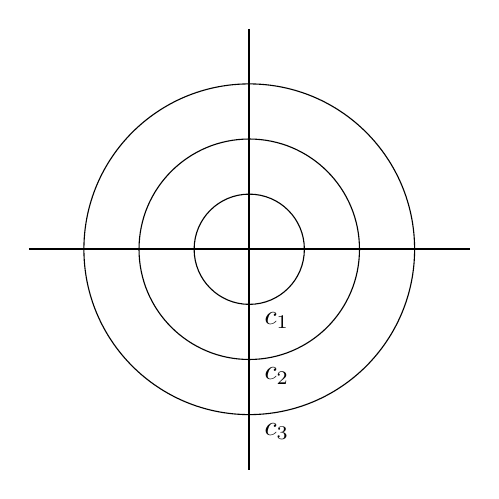
\begin{tikzpicture}[scale=0.7]
        \draw[thick] (-4,0) -- (4,0) (0,4)-- (0,-4);
        \draw (0,0) circle (1)
        (0,0) circle (2)
        (0,0) circle (3);
        \draw (0.5,-1.3) node{$c_1$}
        (0.5,-2.3) node{$c_2$}
        (0.5,-3.3) node{$c_3$};
    \end{tikzpicture}
\end{center}
%circle graph
\noindent \textbf{Formation of Differential Equation} \\ [5pt]
Suppose we are given a \( n \)-parameter family of curves. Then there will be \( n \) arbitrary constants occurring in the given family of curves. Then we can obtain on \( n \)th-order differential equation whose solution is the given family as follows. \\ [5pt]
Differential the given equation of the family of curves \( n \) times so as to get the \( n \) additional equation containing n arbitrary constant and derivatives.Then eliminate the n arbitrary constant to get the required DE.

\vspace{1em}
\begin{tcolorbox}[breakable, title = {\textbf{Example 1.7: Find the D.E of the relation $y = Ae^{2x} + Be^{-2x} $, where A, B are constants.}}]
    \textbf{Solution : }
\[
y = Ae^{2x} + Be^{-2x}
\quad \Rightarrow \quad \frac{dy}{dx} = 2Ae^{2x} - 2Be^{-2x}\]
\[
\quad \Rightarrow \quad \frac{d^2y}{dx^2} = 4(Ae^{2x} + Be^{-2x}) = 4y
\]

\[
\Rightarrow \quad \frac{d^2y}{dx^2} - 4y = 0
\]

\end{tcolorbox}

 \begin{tcolorbox}[breakable, title = {\textbf{Example 1.8: Find the DE of the relation \( y = (c + x)^2 \)}}]
    \textbf{Solution : }

\[
y = (c + x)^2
\quad \Rightarrow \quad \frac{dy}{dx} = 2(c + x)
\]
\[
\left( \frac{dy}{dx} \right)^2 = 4(c + x)^2 = 4y
\quad \Rightarrow \quad \left( \frac{dy}{dx} \right)^2 - 4y = 0
\]
 \end{tcolorbox}
\begin{tcolorbox}[breakable, title = H.W:]
    \begin{enumerate}
    \item Find the D.E of the family of curves $y=e^x(A\cos x+B\sin x)$ where $A$ and $B$ are constants. 
    \item Find the D.E for the family of curves $xy=c^{(3cx-1)}$
    \item Verify that \vspace*{-10pt}
    \begin{enumerate}
        \item $\,\,y=c_1e^{2x}+c_2e^{2x}$ is a solution of D.E: $\dfrac{d^2y}{dx^2}-4\dfrac{dy}{dx}+4y=0$  
    \end{enumerate}
\end{enumerate}
\end{tcolorbox}

\noindent \textbf{Initial Value Problem: } 
\begin{adjustwidth}{1.5cm}{0pt}
    $\dfrac{dy}{dx}=x$ \\ 
    $\Rightarrow y = \dfrac{x^2}{2}+c$
\end{adjustwidth}
A D.E together with an initial condition is called on initial value problem (IVP) with $x$ as the independent variable it is of the form $y' = \dfrac{dy}{dx} = f'(x,y);\quad y(x_0) = y_0;$ \\ [5pt]
Where $x_0,y_0$ are given values. The initial condition $y(x_0)=y_0$ is used to determine a value of constant is the GS. \\ [5pt]
Example: 
\begin{align*}
    &\dfrac{dy}{dx} = y; \quad y(0) = 3 \\ 
    \Rightarrow \,\, & \int \dfrac{dy}{y} = \int dx \\ 
    \Rightarrow\,\, & \ln y = x+c \\ 
    \Rightarrow \,\, &y = e^{(x+c)} \\ 
    \text{At }  x&=0, y =3 \\ 
    3 &= e^{(0+c)} = e^c \\ 
    \text{So, }y &= 3e^x
\end{align*}
\begin{flushright}
    {\small \textbf{End of Class 02 (12 Aug,2025)}}
\end{flushright}
\newpage
\noindent\textbf{\large Existence and Unique Solution} 
$$y = x^n$$
\begin{center}
    $x\uparrow y\uparrow$ but when $0 < x < 1$ then $x\uparrow y\downarrow$
\end{center}
\fbox{\strut $\dfrac{dy}{dx} = f(x,y) ; y(x) = y_0$} $\longrightarrow$ initial value \\
If $f(x,y)$ and $\dfrac{dy}{dx}$ are continuous on $\mathbb{R}$
%Some part Gap




\begin{tcolorbox}[breakable, title = {\textbf{Example 1.9: } Solve $x\dfrac{dy}{dx} = y;\quad  y(0) = 1$}]
    Solution: 
    \vspace*{-15pt}
    \begin{adjustwidth}{2cm}{0pt}
        \begin{flalign*}
    &x\dfrac{dy}{dx} = y& \\ 
    \Rightarrow \,\, &\dfrac{dy}{dx} = \dfrac{y}{x} = f(x,y); \qquad y(0) = 1 \quad (0,1) &\\
    \Rightarrow \,\,&\dfrac{dy}{y} = \dfrac{dx}{x} \\
    \Rightarrow \,\, &\ln y = \ln x + \ln c&\\ 
    \Rightarrow \,\, &\ln y = \ln (xc) &\\ 
    \Rightarrow \,\, &y = xc&
   \end{flalign*} 
    \end{adjustwidth}
When $x = 0$, $$1=0\cdot c \qquad [y(0)=1]$$ 
There is no solution in $(0,1).$ \\
When $x=0, y(0)=c\cdot 0 = 0$, but given that at $x=0; y =1.$ This is shows that the solution doesn't satisfy the initial condition. \\
So, the given IVP $x\dfrac{dy}{dx} = y; y(0)=1$ has no solution. \\
Since $f(x,y) = \dfrac{y}{x}$ is not cont's at (0,1).  
\end{tcolorbox}
\begin{tcolorbox}[breakable, title = {\textbf{Example 1.10: } Solve $x\dfrac{dy}{dx} = y;\quad  y(1) = 1$}]
    Solution:  
    \vspace*{-15pt}
    \begin{adjustwidth}{2cm}{0pt}
        \begin{flalign*}
            &x\dfrac{dy}{dx} = y& \\ 
            \Rightarrow \,\, &\dfrac{dy}{dx} = \dfrac{y}{x} = f(x,y)& \\ 
            \Rightarrow \,\, &\dfrac{df}{dy} = \dfrac{1}{x} &
        \end{flalign*}
    \end{adjustwidth}
    Since $f(x,y)$ and $\dfrac{df}{dy}$ both are continuous at $(1,1)$. So, this IVP has a unique solution. 
    \begin{adjustwidth}{2cm}{0pt}
        \begin{flalign*}
            &\dfrac{dy}{dx} = \dfrac{y}{x}& \\
            \Rightarrow \, \, &\dfrac{dy}{y}=\dfrac{dx}{x}& \\
            \Rightarrow \,\, &\ln y = \ln x + \ln c&\\ 
            \Rightarrow \,\, &\ln y = \ln (xc) &\\ 
            \Rightarrow \,\, &y = xc&
        \end{flalign*}
    \end{adjustwidth}
    When $x=1; y= 1 = c\cdot 1 \Rightarrow c = 1;$ \\
    So, $y = x$ is the unique solution of the given IVP. \\
    \hspace*{20pt} \fbox{\strut $y = cx$}$\longrightarrow$ G.S \\
    \hspace*{23pt} \fbox{\strut $y = x$}$\longrightarrow$ P.S  
\end{tcolorbox}
\begin{tcolorbox}[breakable, title = {\textbf{Example 1.11: } Solve $x\dfrac{dy}{dx} = y;\quad  y(0) = 0$}]
    Solution:  
    \vspace*{-15pt}
    \begin{adjustwidth}{2cm}{0pt}
        \begin{flalign*}
            &\dfrac{dy}{dx} = \dfrac{y}{x}& \\
            \Rightarrow \, \, &\dfrac{dy}{y}=\dfrac{dx}{x}& \\
            \Rightarrow \,\, &\ln y = \ln x + \ln c&\\ 
            \Rightarrow \,\, &\ln y = \ln (xc) &\\ 
            \Rightarrow \,\, &y = xc&
        \end{flalign*}
    \end{adjustwidth}
    When $x=0; y= 0 = c\cdot 0 \Rightarrow c = 0;$ \\
    The solution of the given IVP is exist but not unique solution (it has many solution). 
\end{tcolorbox}
\noindent Therefore, the IVP $\dfrac{dy}{dx} = \dfrac{y}{x}; \quad y(x_0) = y_0$ has
\begin{enumerate}
    \item no solution if $x_0 = 0, y_0 \neq 0$ 
    \item unique solution if $x_0 \neq 0; y \subset \mathbb{R} \quad [y(1)=1]$
    \item Infinity many solutions if $x_0 =0, y_0 = 0$.
\end{enumerate}
\textbf{\large Equation of $1^{st}$ order and $1^{st}$ degree} \\ [5pt]
There are two standard form of the differential equation of $1^{st}$ order and $1^{st}$ degree namely.
\begin{enumerate}
    \item $\dfrac{dy}{dx}=f(x,y) \longrightarrow$ Derivative from separable of variables. 
    \item $M(x,y)dx+N(x,y)dy=0 \longrightarrow $ Differential form  
\end{enumerate}
If a DE of the $1^{st} order$ and $1^{st}$ degree is of the form $f_1(x)dx = f_2(x)dy
$ where $f_1(x)$ is a function of $x$ only and $f_2(y)$ is a function of $y$ only. 

% Space for Example and remaining part 

\begin{tcolorbox}[breakable, title = {\textbf{Example 1.12: }Solve the D.E $(1+x^2)(1+y^2)dx-xydy=0$}]
Solution: 
\begin{adjustwidth}{1cm}{0pt}
    \vspace*{-15pt}
    \begin{flalign*}
        &\dfrac{(1+x^2)(1+y^2)dx}{x(1+y^2)}-\dfrac{xy}{x(1+y^2)}dy = 0 \quad \text{[Divided by $x(1+y^2)$]}& \\ 
        \Rightarrow \,\, & \dfrac{(1+x^2)}{x}dx-\dfrac{y}{(1+y^2)dy} = 0& \\ 
        \Rightarrow\,\, & \left(\dfrac{1}{x}+x\right)dx - \left(\dfrac{y}{1+y^2}\right)dy = 0& \\ 
        \Rightarrow\,\, &\left(\ln x+\dfrac{x^2}{2}\right)-\dfrac{1}{2}\ln (1+y^2) = c&  \\ 
        \Rightarrow\,\, &2\ln x+x^2-\ln (1+y^2) = 2c = c& \\
        \Rightarrow\,\, &\ln x^2+x^2-\ln (1+y^2) = c& \\ 
        \Rightarrow\,\, &\ln \dfrac{x^2}{1+y^2} = c -x^2& \\ 
        \Rightarrow\,\, &\dfrac{x^2}{1+y^2} = e^{c-x^2}& \\
        \Rightarrow\,\, &\dfrac{x^2}{e^{c-x^2}}=1+y^2& \\ 
        \Rightarrow\,\, &1+y^2 = \dfrac{x^2e^{x^2}}{c}&
    \end{flalign*}
\end{adjustwidth}
\end{tcolorbox}
\begin{flushright}
    {\small \textbf{End of Class 03 (19 Aug,2025)}}
\end{flushright}
\begin{tcolorbox}[breakable, title = {\textbf{Example 1.13: }Solve $\dfrac{dy}{dx}=\sin(x+y)+\cos(x+y)$}]
Solution: \\
Let, 
\begin{adjustwidth}{1cm}{0pt}
    \vspace*{-15pt}
    \begin{flalign*}
        &x+y=z&\\
        \Rightarrow\,\, &1+\dfrac{dy}{dx} = \dfrac{dz}{dx}& \\ 
        \Rightarrow\,\, &\dfrac{dy}{dx} = \dfrac{dz}{dx}-1& 
    \end{flalign*}
    \begin{flalign*}
        (i)\,\, &\dfrac{dz}{dx}-1=\sin (z)+\cos (z)& \\ 
        \Rightarrow\,\, &\dfrac{dz}{dx} = \sin(z)+\cos(z)+1& \\
        \Rightarrow\,\, &\dfrac{dz}{\sin z+\cos z+1} = dx& \\
        \Rightarrow\,\, &\dfrac{dz}{2\cos ^2\dfrac{z}{2}+2\sin\dfrac{z}{2}\cos\dfrac{z}{2}} = dx& \\
        \Rightarrow\,\, &\dfrac{\dfrac{dz}{\cos^2\dfrac{z}{2}}}{2+2\tan\dfrac{z}{2}} = dx& \\
        \Rightarrow\,\, &\dfrac{\dfrac{1}{2}\sec^2\dfrac{z}{2}}{1+\tan\dfrac{z}{2}}dz = dx& \\
        \Rightarrow\,\, &\ln \left(1+\tan\dfrac{z}{2}\right) = x+c \\
        \Rightarrow\,\, &\ln \left(1+\tan\dfrac{x+y}{2}\right) = x+c
    \end{flalign*}
\end{adjustwidth}
\end{tcolorbox}
\begin{tcolorbox}[breakable, title= \textbf{H.W: }]
    Solve the following D.E: 
    \begin{enumerate}
        \item $2xdy-2ydz=\sqrt{x^2+4y^2}dx$
        \item $(3y-7x+7)dx+(7y-3x+3)dy=0$
    \end{enumerate}
\end{tcolorbox}
\textbf{\large Homogenous function: }\\ [5pt]
Function $z=f(x,y)$ is called homogenous function of degree $n$ if $f(xt, yt) = t^nf(x,y)=x^n\phi\left(1,\dfrac{y}{x}\right)$. \\ [5pt]
Example: \\
\vspace*{-20pt}
\begin{center}
    \begin{minipage}{0.4\linewidth}
        \vspace*{-5pt}
    \begin{flalign*}
        f(x,y) &= x^2+2xy+y^2& \\
        f(xt,yt) &= (xt)^2+2(xt)(yt)+(yt)^2 & \\ 
        &=t^2(x^2+2xy+y^2)& \\
        &=t^2f(x,y)&
    \end{flalign*}
\end{minipage}
\begin{minipage}{0.09\linewidth}
    \begin{center}
        \vspace*{10pt}
        \rule{1pt}{2.8cm}
    \end{center}
\end{minipage}
\begin{minipage}{0.4\linewidth}
    \begin{flalign*}
        f(x,y) &= x^2+2xy+y^2& \\
        &= x^2\left(1+2\cdot1\cdot\dfrac{y}{x}+\dfrac{y^2}{x^2}\right)& \\ 
       &=x^2\phi\left(1,\dfrac{y}{x}\right)&
    \end{flalign*}
\end{minipage}
\end{center}
A D.E of the form - $M(x,y)dx+N(x,y)dy=0$ is said to be homogenous if both the co-efficient $M(x,y)$ and $N(x,y)$ are homogenous function of same degree. \\
Example: \begin{enumerate}
    \item $2xydx+s^2dy=0$
    \item $(x^2+xy)dx+(y^2+xy)dy=0$
\end{enumerate}
In other words $M(x,y)dx+N(x,y)dy=0$ is homogenous D.E of degree $n$ if $M(xt,yt)=t^nM(x,y)$ and $N(xt,yt)=t^nN(x,y)$. \\ [5pt]
$\dfrac{dy}{dx} = - \dfrac{M(x,y)}{N(x,y)} = \dfrac{f_1(x,y)}{f_2(x,y)}$ \\ [5pt]
A D.E of the form $\dfrac{dy}{dx}=\dfrac{f_1(x,y)}{f_2(x,y)}$ in which $f_1(x,y)$ and $f_2(x,y)$ are homogenous function of same degree can be reduced to an equation in which variables are separated by using $y=vx$ or $x=vy$ in this case, our new variables are $v,x$ or $v,y$
\begin{tcolorbox}[breakable, title = {\textbf{Example 1.14: }Solve the D.E $(x^3+3xy^2)dx+(y^3+3x^2y)dy=0$}]
Solution:
\begin{adjustwidth}{1cm}{0pt}
    \vspace*{-20pt}
    \begin{flalign*}
        &(x^3+3xy^2)dx+(y^3+3x^2y)dy=0& \\
        \Rightarrow\,\, &\dfrac{dy}{dx} = -\dfrac{x^2+3xy^2}{y^3+3x^2y} = -\dfrac{x^3\left(1+\left(\dfrac{y}{x}\right)^2\right)}{x^3\left(\left(\dfrac{y}{x}\right)^3+3\left(\dfrac{y}{x}\right)\right)}& \\ 
        \Rightarrow\,\, &\dfrac{dy}{dx} = -\dfrac{1+\left(\dfrac{y}{x}\right)^2}{\left(\dfrac{y}{x}\right)^3+3\left(\dfrac{y}{x}\right)} \qquad \longrightarrow (i)&
    \end{flalign*}
\end{adjustwidth}
Now let, $$y=vx \quad  \Rightarrow v = \dfrac{y}{x}$$
$$\dfrac{dy}{dx}= v+x\dfrac{dv}{dx}\quad \longrightarrow(ii)$$
Using the equation $(i)$ and $(ii)$,
\begin{adjustwidth}{1cm}{0pt}
    \vspace*{-20pt}
    \begin{flalign*}
        v+x\dfrac{dv}{dx} &=  -\dfrac{1+3v^2}{v^3+3v}& \\
        \Rightarrow\,\, x\dfrac{dv}{dx} &= -\dfrac{1+3v^2}{v^3+3v}-v& \\ 
        &=\dfrac{-1-3v^2-v^4-3v^2}{v^3+3v}& \\
        &=\dfrac{-1-6v^2-v^4}{v^3+3v}& \\
        &=-\dfrac{v^4+6v^2+1}{v^3+3v}& \\ 
        \Rightarrow\,\, -\dfrac{v^3+3v}{v^4+6v^2+1}dv &= \dfrac{1}{x}dx \\ 
        \Rightarrow\,\, -\dfrac{4(v^3+3v)}{v^4+6v^2+1}dv &= 4\dfrac{1}{x}dx \\
        \Rightarrow\,\, -\ln(v^4+6v^2+1) &= 4\ln x +\ln c  \\ 
        \Rightarrow \,\, \ln\left(\left(\dfrac{y}{x}\right)^4+6\left(\dfrac{y}{x}\right)^2+1\right)^{-1} &= \ln (x^4c) \\ 
        \Rightarrow\,\, \dfrac{1}{\left(\dfrac{y}{x}\right)^4+6\left(\dfrac{y}{x}\right)^2+1}. &=x^4c \\
        \Rightarrow\,\,
        \dfrac{1}{c} &= x^4\left(\left(\dfrac{y}{x}\right)^4+6\left(\dfrac{y}{x}\right)^2+1\right) \\ 
        \Rightarrow\,\, c &= y^4+6x^2y^2+x^4
    \end{flalign*}
\end{adjustwidth}
\end{tcolorbox}


\begin{tcolorbox}[breakable, title = {\textbf{Example 1.15: }Solve the D.E $(x^2+y^2)dx+2xydy=0$}]
Solution:
\begin{adjustwidth}{1cm}{0pt}
    \vspace*{-20pt}
    \begin{flalign*}
        \dfrac{dy}{dx} = \dfrac{x^2+y^2}{2xy} \qquad \longrightarrow (i)
    \end{flalign*}
\end{adjustwidth}
Now let, $$y=vx \quad  \Rightarrow v = \dfrac{y}{x}$$
$$\dfrac{dy}{dx}= v+x\dfrac{dv}{dx}\quad \longrightarrow(ii)$$
Using the equation $(i)$ and $(ii)$,
\begin{adjustwidth}{1cm}{0pt}
    \vspace*{-20pt}
    \begin{flalign*}
        v+x\dfrac{dv}{dx} &= -\dfrac{x^2+v^2x^2}{2x\cdot vx}& \\
        \Rightarrow \,\, x\dfrac{dv}{dx} &= -\dfrac{1+v^2}{2v}-v = \dfrac{-1-v^2-2v^2}{2v} =- \dfrac{1+3v^2}{2v}&\\
        \Rightarrow\,\,-\dfrac{2vdv}{1+3v^2} &=\dfrac{1}{x}dx& \\
        \Rightarrow\,\, \dfrac{6vdv}{1+3v^2} &= -\dfrac{3}{x}dx & \\ 
        \Rightarrow \ln (1+3v^2) &= -3\ln x-\ln c = -\ln (x^3c) = \ln \left(\dfrac{1}{x^3c}\right)& \\ 
        \Rightarrow\,\, 1+3v^2 &= \dfrac{1}{x^3c}& \\
        \Rightarrow\,\, 1+3\left(\dfrac{y}{x}\right)^2 &= \dfrac{1}{x^3c}& \\
        \Rightarrow\,\, x^3+3xy^2 &=c&
\end{flalign*}

\end{adjustwidth}
\end{tcolorbox}

\end{document}